\documentclass[class=report, float=false, crop=false]{standalone}

\usetheme{Warsaw}
% \usecolortheme{spruce}

%%%%% PACKAGES

\usepackage{graphicx} % figures
\usepackage{multimedia} % videos
\usepackage{url}
\usepackage{amsmath}
\usepackage{amssymb}
\everymath{\displaystyle}
\usepackage{epstopdf} % conversion from .eps to .pdf
\usepackage[utf8]{inputenc}
\usepackage[T1]{fontenc}
\usepackage{upgreek}
\usepackage{nameref}
\usepackage{url}
\usepackage{pgf, tikz}
\usepackage{float}
\usepackage[english]{babel}
\usepackage{caption}
\usepackage{subcaption}
\usepackage{fontawesome5}
\usepackage{xcolor}

\usepackage{biblatex}
\addbibresource{references/biblio.bib}

%%%%% TEMPLATE

\captionsetup{font=scriptsize,labelfont={scriptsize, color=blue}}

\AtBeginSubsection[]
{
 \begin{frame}<beamer>{}
   \tableofcontents[currentsection,currentsubsection]
 \end{frame}
}
\AtBeginSection[]
{
  \begin{frame}<beamer>{}
    \tableofcontents[currentsection]
  \end{frame}
}

\defbeamertemplate*{footline}{mytheme}%
{  \begin{beamercolorbox}[ht=2.5ex]{bordure}
\begin{beamercolorbox}[wd=0.2\paperwidth,ht=2.5ex,dp=1ex,center]{author in head/foot}%
\usebeamerfont{author in head}\insertshortauthor
\end{beamercolorbox}%
\begin{beamercolorbox}[wd=0.57\paperwidth,ht=2.5ex,dp=1ex,center]{title in head/foot}%
\usebeamerfont{title in head/foot}\insertshorttitle
\end{beamercolorbox}%
% \begin{beamercolorbox}[wd=0.4\paperwidth,ht=2.5ex,dp=1ex,center]{title in head/foot}%
% \usebeamerfont{title in head/foot}\insertdate
% \end{beamercolorbox}%
\begin{beamercolorbox}[wd=0.12\paperwidth,ht=2.5ex,dp=1ex,center]{title in head/foot}%
\usebeamerfont{title in head/foot}\insertdate
\end{beamercolorbox}%
\begin{beamercolorbox}[wd=0.11\paperwidth,ht=2.5ex,dp=1ex,center]{date in head/foot}%
\usebeamerfont{date in head/foot}\insertframenumber /\inserttotalframenumber{}\hspace{2ex}
\end{beamercolorbox}%

  \end{beamercolorbox}
}

% \defbeamertemplate*{headline}{mytheme}%
% {  \begin{beamercolorbox}[ht=2.5ex]{bordure}
% \begin{beamercolorbox}[wd=\paperwidth,ht=2.5ex,dp=2ex]{author in head/foot}%
% \usebeamerfont{author in head}\vskip6pt\insertsectionnumber.~\insertsection \hfill \insertsubsection
% \end{beamercolorbox}%
%
%   \end{beamercolorbox}
% }

\makeatletter
\let\insertsupervisor\relax
\newcommand\supervisortitle{supervised by}
\mode<all>
{
  \newcommand\supervisor[1]{\def\insertsupervisor{#1}}
  \titlegraphic{}
}
\defbeamertemplate*{title page}{supdefault}[1][]
{
  \vbox{}
  \vfill
  \begingroup
    \centering
    \begin{beamercolorbox}[sep=8pt,center,#1]{title}
      \usebeamerfont{title}\inserttitle\par%
      \ifx\insertsubtitle\@empty\relax%
      \else%
        \vskip0.25em%
        {\usebeamerfont{subtitle}\usebeamercolor[fg]{subtitle}\insertsubtitle\par}%
      \fi%
    \end{beamercolorbox}%
    \vskip1em\par
    \begin{beamercolorbox}[sep=8pt,center,#1]{author}
      \usebeamerfont{author}\textbf{\insertauthor}
    \end{beamercolorbox}
    \vspace{-10pt}
    \ifx\insertsupervisor\relax\relax\else
    \begin{beamercolorbox}[sep=8pt,center,#1]{author}
      \usebeamerfont{author}{\footnotesize \supervisortitle}~{\small\insertsupervisor}
    \end{beamercolorbox}\fi
    \vspace{-5pt}
    \begin{beamercolorbox}[sep=8pt,center,#1]{date}
      \usebeamerfont{date}\insertdate
    \end{beamercolorbox}\vskip0.5em
    {\usebeamercolor[fg]{titlegraphic}\inserttitlegraphic\par}
  \endgroup
  \vfill
}
\setbeamertemplate{title page}[supdefault][colsep=-4bp,rounded=true,shadow=\beamer@themerounded@shadow]\makeatother

\setbeamerfont{footnote}{size=\tiny}

\makeatletter
\newlength\beamerleftmargin
\setlength\beamerleftmargin{\Gm@lmargin}
\makeatother

%%%%% COMMANDS

\providecommand\blfootnote[1]{%
  \begingroup
  \renewcommand\thefootnote{}\footnote{#1}%
  \addtocounter{footnote}{-1}%
  \endgroup
}

\providecommand\encircle[1]{%
  \tikz[baseline=(X.base)]
    \node (X) [draw, shape=circle, inner sep=0] {\strut #1};}

\providecommand{\appropto}{\mathrel{\vcenter{
  \offinterlineskip\halign{\hfil$##$\cr
    \propto\cr\noalign{\kern2pt}\sim\cr\noalign{\kern-2pt}}}}}

\setbeamertemplate{blocks}[rounded][shadow=true]

\providecommand{\isEquivTo}[1]{\underset{#1}{\sim}}

\providecommand{\appropto}{\mathrel{\vcenter{
  \offinterlineskip\halign{\hfil$##$\cr
    \propto\cr\noalign{\kern2pt}\sim\cr\noalign{\kern-2pt}}}}}

\makeatletter
\providecommand{\subalign}[1]{%
  \vcenter{%
    \Let@ \restore@math@cr \default@tag
    \baselineskip\fontdimen10 \scriptfont\tw@
    \advance\baselineskip\fontdimen12 \scriptfont\tw@
    \lineskip\thr@@\fontdimen8 \scriptfont\thr@@
    \lineskiplimit\lineskip
    \ialign{\hfil$\m@th\displaystyle##$&$\m@th\displaystyle{}##$\crcr
      #1\crcr
    }%
  }
}
\makeatother


\graphicspath{{introduction}}

\begin{document}

\chapter*{Introduction}
\label{introduction}
\addcontentsline{toc}{chapter}{Introduction}

We can distinguish three general classes of non-equilibrium systems \cite{cates2015motility}:
\begin{itemize}
  \item systems relaxing towards equilibrium (\textit{e.g.,} thermal system adapting to its thermostat), even if this relaxation is particularly slow (\textit{e.g.,} glasses),
  \item systems with boundary conditions imposing steady currents (\textit{e.g.,} sheared liquid, metal rod between two thermostats),
  \item and \textit{active matter}.
\end{itemize}
Active matter features systems composed of interacting self-propelled units, \textit{active particles}, each capable of converting stored or ambient free energy into systematic movement \cite{marchetti2013hydrodynamics}. This local energy input, at the origin of self-propulsion, drives the system far from thermodynamic equilibrium \cite{levis2014clustering}. Examples of such materials are ubiquitous in biology and span a great range of length scales, from swarms of bacteria \cite{dombrowski2004self} and cell tissues \cite{angelini2011glass}, to schools of fish \cite{calovi2014swarming} and flocks of birds \cite{cavagna2014bird} (see figure \ref{birds}).\\

\begin{figure}[h!]
\centering
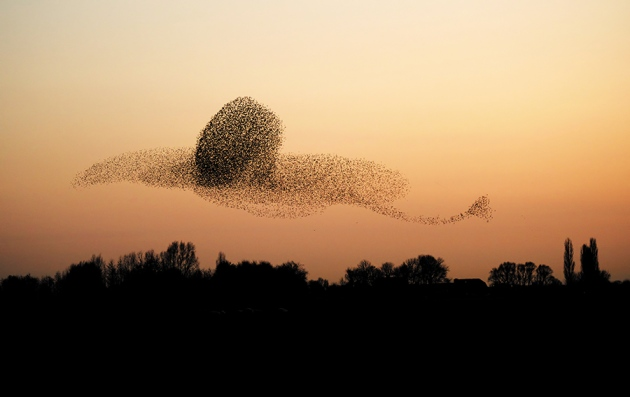
\includegraphics[width=0.8\textwidth]{birds}
\caption{Flocking birds. \textit{source:} Hans Overduin/NIS/Minden/Getty, \cite{popkin2016physics}.}
\label{birds}
\end{figure}

Moreover, in many biological phenomena, colletive motion of cells is of fundamental importance, such as in the healing of wounds \cite{haga2005collective} and cancer propagation \cite{friedl2009collective}, hence motivating fundamental and theoretical research on the topic, jointly between biologists and physicists \cite{garcia2015physics}.\\

From a physicist's point of view, these systems are particulary interesting because they exhibit surprising phenomena, often defying physical intuition, despite being relatively simple in nature. Such phenomena include swarming, clustering, and non-equilibrium kinetic phase transitions \cite{vicsek1995novel, szabo2006phase}. Their study has motivated the development of artificial active particles for experimental purposes \cite{howse2007self, theurkauff2012dynamic}, as well as various computational models \cite{garcia2015physics, vicsek1995novel, levis2014clustering, wysocki2014cooperative, fily2014freezing, redner2013structure}.\\

Our research project, which current development is summarised in the following report, aims at numerically analysing a model system of active matter. This system, inspired by Fily \textit{et al.} \cite{fily2012athermal, fily2014freezing}, consists of Brownian disks with purely repulsive interparticle harmonic potential, each of them performing independent persistent random walks. We will show that despite the simplicity of this model, interesting and surprising phenomena arise: motility-induced phase separation and long-range correlated displacements and shear strain, even at high times. These phenomena will be characterised and compared with current developments in supercooled liquids and glasses research.\\

All computer programs with which the presented results were obtained were developed in Python \faPython~ (and occasionally in bash) and written by the author. All scripts -- for simulation and analysis purposes -- are available in the GitHub \faGithub~ repository \href{https://github.com/yketa/active_particles}{yketa/active\_particles}. This repository is organised such that it can be used as a Python \faPython~ package, usable with the provided Conda environment. Simulations and analyses were performed on the Stewart Blusson Quantum Matter Institute cluster.\\

This report is organised as follows. In \hyperref[chap:model]{chapter \ref{chap:model}}, we describe our model system, as well as the methods we have used in our simulations. We then review 3 important phenomena observed in our simulations. In \hyperref[chap:mips]{chapter \ref{chap:mips}}, we characterise the motility-induced phase separation. In \hyperref[chap:displacement]{chapter \ref{chap:displacement}}, we study the displacement correlations. And in \hyperref[chap:strain]{chapter \ref{chap:strain}}, we study the shear strain correlations. In each part, we provide details on the implementation of every calculations.

\end{document}
